\chapter{Ход работы}
\label{ch:chap2}

\section*{\textbf{Введение}}

В этой лабораторной работе необходимо смоделировать СМО разных типо: M/M/1, M/G/1, G/M/1, G/G/1, расчитать их характеристики 
и визуализировать их.

\section*{\textbf{Функция для расчета характеристик СМО}}

Вычисления производились по формулам Хинчина-Полячека. Формулы для расчета характеристик могут разниться для каждого из типа СМО.
Для типов G/M/1, G/G/1 формулы не предусмотрены, но есть сторонние функции, аппроксимирующие значение, но я их не рассматривал.

\begin{lstlisting}
function stats = MG1_param(tn, c, p)
    %N_q - avg queue len
    %N - avg tasks count in system
    %W - avg waiting time 
    %T - avg time task into system
    %t_n - set of time serving

    %avg time serving
    avg_tn = mean(tn);

    %compute params
    stats.N_q = p^2 * (1 + c) / (2*(1-p));
    stats.N = p + stats.N_q;
    stats.W = p * avg_tn * (1 + c) / (2*(1-p));
    stats.T = avg_tn + stats.W;

end
\end{lstlisting}

\begin{lstlisting}
function stats = MM1_param(tn, p)
    %N_q - avg queue len
    %N - avg tasks count in system
    %W - avg waiting time 
    %T - avg time task into system
    %t_n - set of time serving

    %avg time serving
    avg_tn = mean(tn);

    %compute params
    stats.N_q = p^2/(1-p);
    stats.N = p / (1 - p);
    stats.W = stats.N * avg_tn;
    stats.T = avg_tn / (1-p);
end
\end{lstlisting}

\begin{figure}[H]
    \centering
    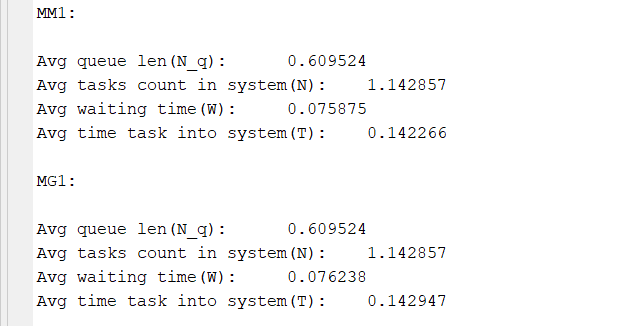
\includegraphics[width=1.0\textwidth]{param.png}
    \caption{Параметры СМО}
\end{figure}

\section*{\textbf{Визуализация поступления заявок и их обработки}}

СМО характеризуются управляющими последовательностями $t_n$ - временные интервалы поступления заявок, $v_n$ - временные интервалы
обработки заявок. Эти последовательности могут быть распределны по разным законам. Исходя из этих последовательностей можно узнать,
как поступали заявки и как они обрабатывались в зависимости от времени, найти кол-во заявок в СМО в текущий момент времени.

\begin{lstlisting}
function t = system_param(tn, vn, type)
    
    %сортируем и накапливаем сумму
    vn = cumsum(vn);
    tn = cumsum(tn);
    
    %визуализация
    figure;
    plot(tn, 0:1:length(tn) - 1);
    hold on;
    plot(vn, 0:1:length(vn) - 1);
    title(sprintf("Зависимость числа пришедших/обработанных заявок от времени (%s)", type));
    xlabel("Время,с");
    ylabel("Кол-во заявок,шт");
    hold off;
    grid on;
    legend("Пришедшие заявки", "Обслуженные заявки");
    
    % кол-во заявок в системе
    tasks_in_system = zeros(length(vn), 1);
    
    for i = 1:length(vn)
        tasks_in_system(i) = vn(i) - tn(i); 
    end
    
    figure;
    plot(vn, tasks_in_system);
    title(sprintf("Зависимость кол-ва заявок в системе от времени (%s)", type));
    xlabel("Время,с");
    ylabel("Кол-во заявок,шт");
    t = 1;
end

\end{lstlisting}

Это функция, которая расчитывает и визуализиурет характеристки, указанные выши. Она принимает распределения поступления и обработки
заявок. Аккумулирующая сумма происходит для того, чтобы найти, в какой момент времени пришла/обработалась заявка. Допустим,  $v_N
= [0.2, 0.35, 0.05]$, значит, первая заявка поступила в момент времени 0.2, вторая - в 0.55, третья - 0.6. Далее на графики
выводится зависимость числа пришедших/обработанных заявок от времени и кол-во заявок в системе.


\section*{\textbf{Результаты}}

\begin{figure}[H]
    \centering
    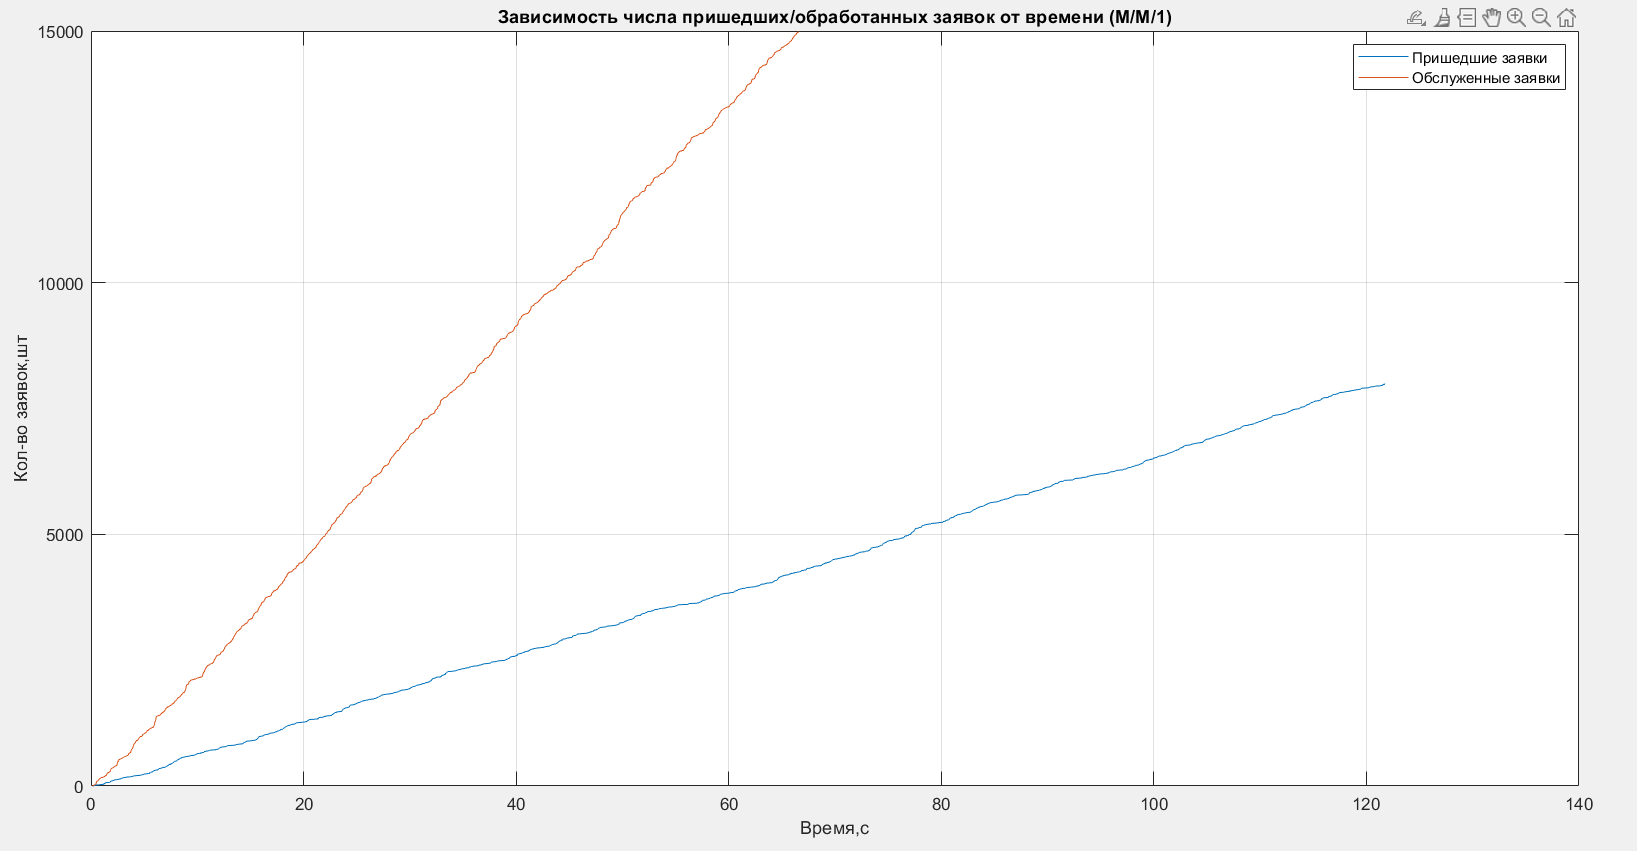
\includegraphics[width=1.0\textwidth]{mm1.png}
    \caption{Зависимость поступления/обработки заявок от времени}
\end{figure}

Можем видеть, что кол-во поступающих заявок и обработанных возрастает с течением времени, что логично. Скорость обработки превышает
скорость поступления заявок.

\begin{figure}[H]
    \centering
    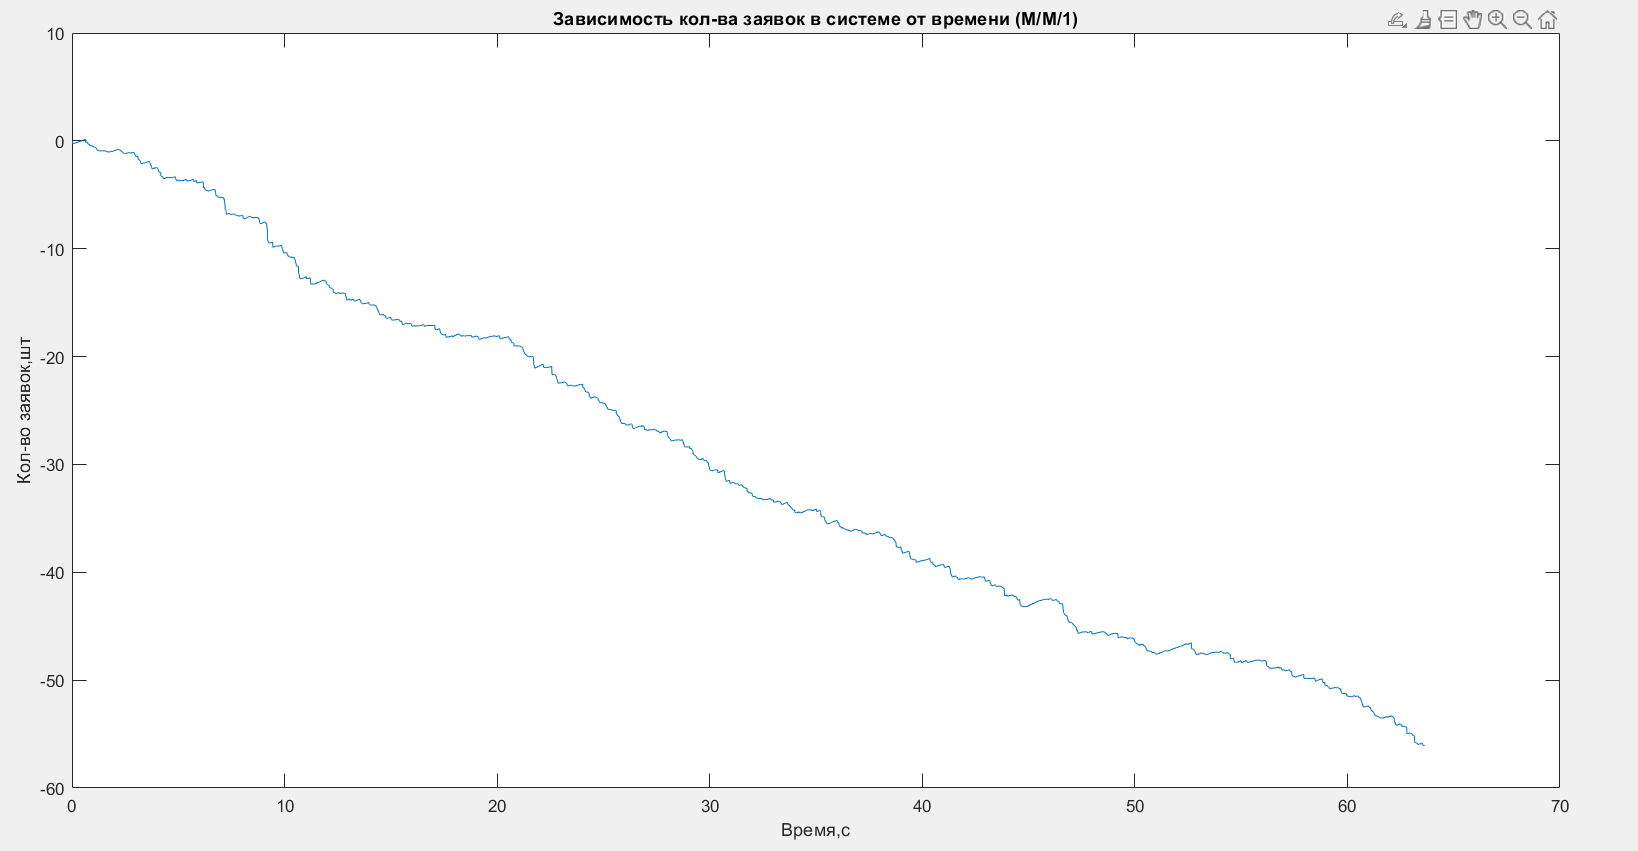
\includegraphics[width=1.0\textwidth]{mm1insys.png}
    \caption{Зависимость кол-ва заявок в системе}
\end{figure}

Из-за того, что скорость постулпения заявок ниже, чем скорость обработки, кол-во заявок в системе стало отрицательным. Отрицательные
значения говорят о том, что в системе нет заявок (потому что они сразу же обрабатываются).

\begin{figure}[H]
    \centering
    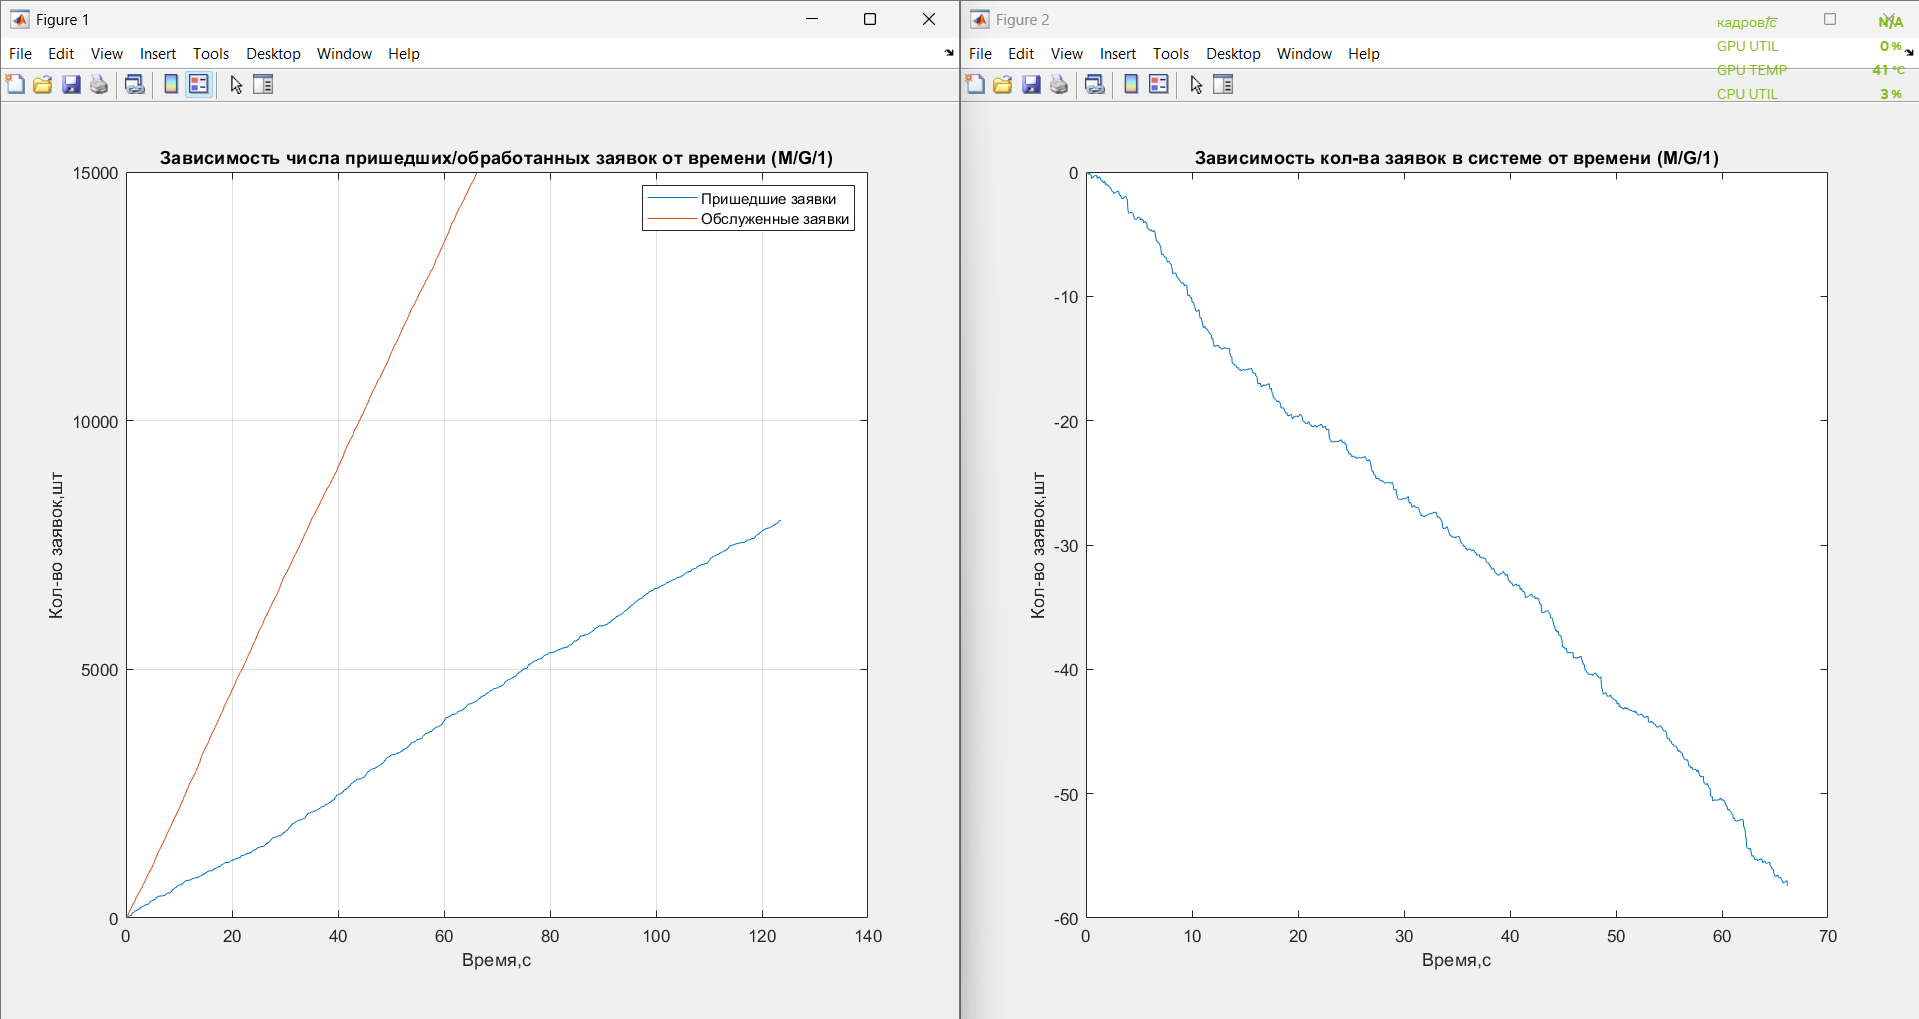
\includegraphics[width=1.0\textwidth]{MG1.png}
    \caption{Характеристики СМО в зависимости от времени}
\end{figure}

Ситуация идентична предыдущей. В качестве G распределения я взял гамма распределение.

\begin{figure}[H]
    \centering
    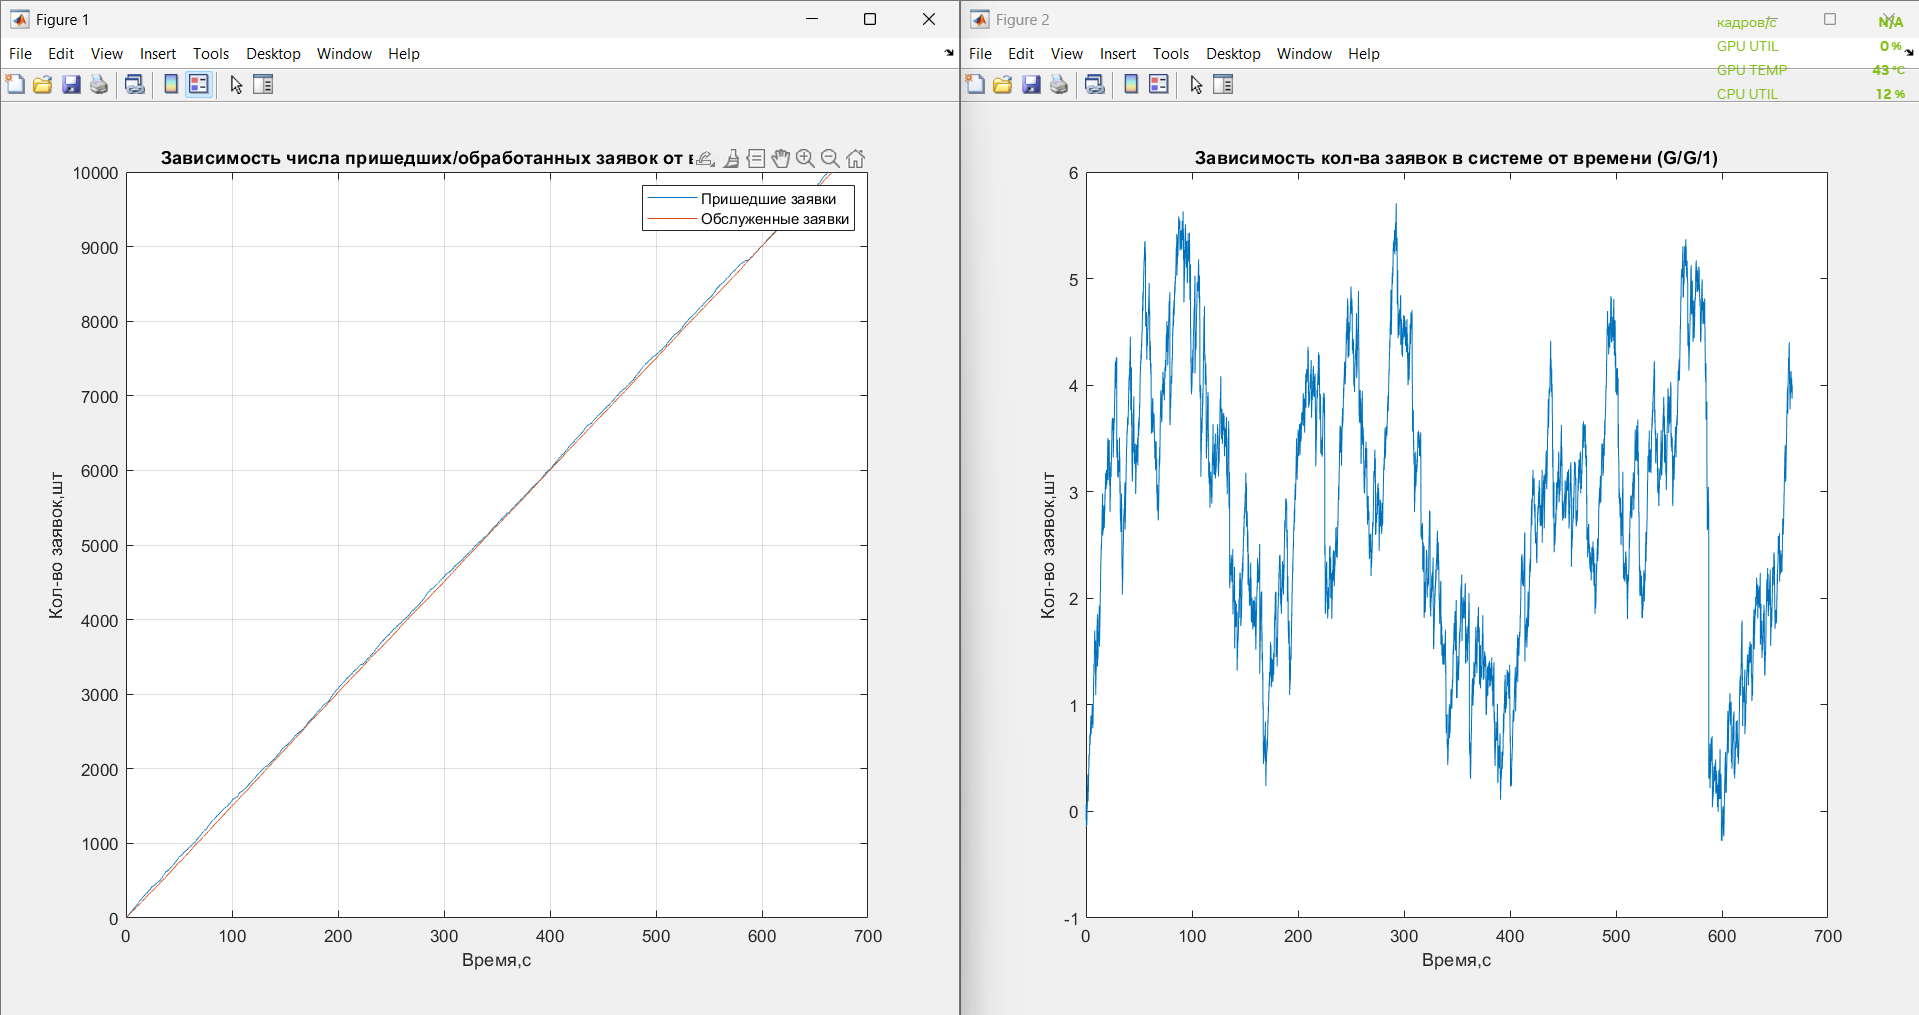
\includegraphics[width=1.0\textwidth]{GG1.png}
    \caption{Характеристики СМО в зависимости от времени}
\end{figure}

Здесь ситуация получилась более интересная. Я взял логнормальное распределение в качестве $v_n$ и экспоненциальное в качестве $t_n$.
На графике слева можем видеть, что иногда кол-во обработанных сообщений становится меньше кол-ва пришедших. Это отражается на графике
справа: если график убывает, то система успевает обработать все заявки и заявок в системе нет. Если график возрастает, то заявок
слишком много и они начинаются копиться в системе.

\section*{\textbf{Контрольные вопросы}}

\begin{figure}[H]
    \centering
    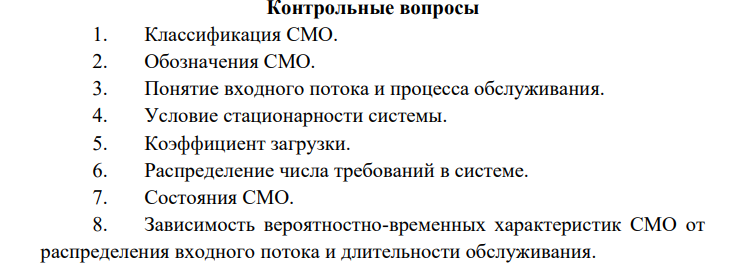
\includegraphics[width=1.0\textwidth]{cq.png} 
    \caption{Контрольные вопросы}
\end{figure}

\begin{enumerate}
    \item 
        \begin{figure}[H]
        \centering
        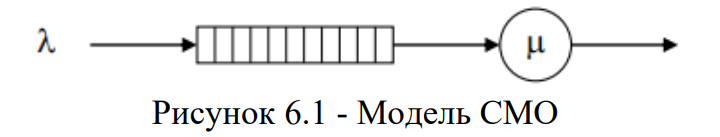
\includegraphics[width=1.0\textwidth]{SMO.png}
        \caption{Обозначение СМО}
        \end{figure}
    \item СМО классифицируются по распределению времени между поступлениями, распределению времени обслуживания, кол-ву обслуживающих устройств.
    \item Входным потоком СМО можно считать поток заявок или поток временных интервалов, в которые приходит заявка.
    \item Стационарность СМО зависит зависит от параметров $\lambda$ и $u$. Если $\lambda$ > $u$, то система не будет стационарной.
    \item Коэффициент загрузки $p = \frac{\lambda}{u}$ показывает, во сколько раз интенсивность поступления заявок больше интенсивности их обработки, если такой коэффициент меньше единицы, то система будет успевать обрабатывать входной поток и заявки не будут копиться в системе.
    \item Закон, по которому распределены управляющие последовательности.
    \item Число заявок, находящихся в системе в данный момент времени (в очереди и на обслуживании).
    \item Тип распределения влияет на характер управляющих последовательностей. Допустим, при одинаковом мат.ожидании экспоненциальное 
    распределение менее стабильную последовательность, чем гамма-распределение. Эти скачки отразятся на скорости работы СМО и длине ее очереди.
\end{enumerate}
   

\endinput
